\documentclass[12pt]{article}
\usepackage{latexsym}
\usepackage{amssymb,amsmath}
\usepackage[pdftex]{graphicx}
\usepackage{color}
\usepackage{epstopdf}


\topmargin = 0.1in \textwidth=5.7in \textheight=8.6in

\oddsidemargin = 0.2in \evensidemargin = 0.2in

\begin{document}

\begin{center}
COMPUTER SCIENCE 20, SPRING 2014 \\
Module \#19 (Undirected Graphs) - checkin \\
Author: Tawheed Abdul-Raheem
\end{center}




\begin{enumerate}

%\item Prove that if a simple graph has more than two nodes and is bipartite, then it cannot be complete. Draw the simple graph that has exactly two nodes and is both bipartite and complete.


%\item We used directed graphs, not simple graphs, to represent relations because relations are inherently directional. If we tried to use simple graphs to represent relations, we would not be able to represent all relations. We can explore this by thinking about converting a simple graph into a digraph by replacing each undirected edge with a pair of opposite-pointing directed edges. If we did this, which of the following could we not possibly represent with digraphs constructed in this way? (Assume that we only consider graphs will at least one edge).
%\begin{enumerate}
%\item symmetric relations

%\item reflexive relations

%\item transitive relations

%\item equivalence relations

%\end{enumerate}

\item Determine which among the four graphs pictured below are isomorphic.  If two of these graphs are
isomorphic, describe an isomorphism between them.  If they are not,
give a property that is preserved under isomorphism such that one
graph has the property, but the other does not.

\begin{center}
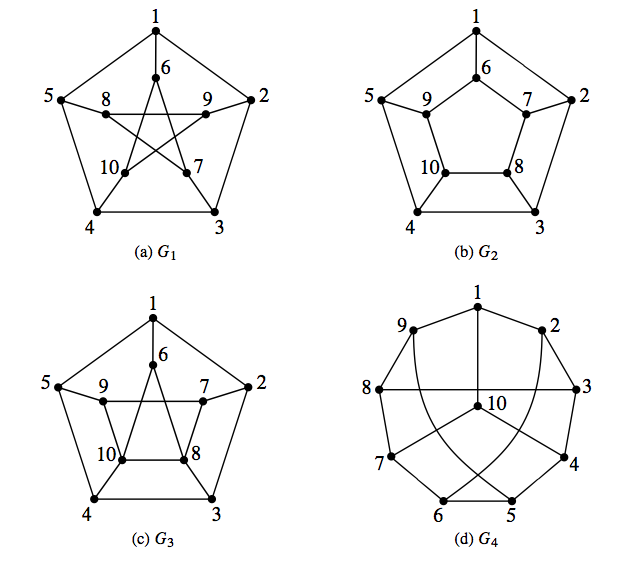
\includegraphics[scale=0.35]{all.png}
\end{center}


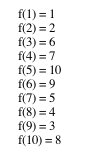
\includegraphics[scale=1.39]{q.png}

%$G(3)$ is not isomorphic with the other graphs because of the number of degree of edges. Below is table showing the degree vertex of each of the graph
%\begin{displaymath}
%\begin{array}{|c|c|c|c|c|}
    %Node & \text{G(1) Degree Vertex} &  \text{G(2) Degree Vertex} & G(3) \text{Degree Vertex} & G(4) \text{Degree Vertex} \\
%\hline
%1 & 3  & 3 & 3 & 3  \\
%2 & 3  & 3 & 3 & 3  \\
%3 & 3  & 3 & 3 & 3  \\
%4 & 3  & 3 & 3 & 3  \\
%5 & 3  & 3 & 3 & 3  \\
%6 & 3  & 3 & 3 & 3  \\
%7 & 3  & 3 & 3 & 3  \\
%8 & 3  & 3 & 4 & 3  \\
%9 & 3  & 3 & 3 & 3  \\
%10 & 3  & 3 & 4 & 3  \\
%\end{array}
%\end{displaymath}

%\item Prove that isomorphism of graphs is an equivalence relation.

%\item Prove that any simple graph with at least two vertices has at least two vertices of the same degree.
\end{enumerate}

\end{document}
